\chapter{Compiler Flags}

In this assignment, different compiler optimization flags for Intel ICC compiler were compared based on how they affect the MFLOPS performance of the Jacobi relaxation method used to solve the stationary 2D heat equation.

Different levels of optimization were examined using the flags \texttt{-O1, -O2, -O3 and -Ofast}\footnote{
    \url{https://www.intel.com/content/www/us/en/docs/cpp-compiler/developer-guide-reference/2021-10/overview.html}
}.
Additionally, specific flags that enable the compiler to perform more aggressive optimizations were considered:
\begin{itemize}
    \item \texttt{-ipo}: Enables interprocedural optimization between files.
    \item \texttt{-fno-alias}: Assert there is no aliasing of memory references, that is, the same memory location is not accessed via different arrays or pointers.
    \item \texttt{ivdep}: Instructs the compiler to ignore assumed vector dependencies.
\end{itemize}
as well as platform specific optimization flags:
\begin{itemize}
    \item \texttt{-xhost}: Tells the compiler to generate instructions for the highest instruction set available on the compilation host processor.
    \item \texttt{-xCORE-AVX512}: Enables the generation of AVX-512 instructions. Leverages wide vector operations.
    \item \texttt{-qopt-zmm-usage mean}: Defines a level of ZMM registers usage.
\end{itemize}

The Intel compiler also provides detailed optimization reports when using the option \texttt{-opt-report}, specifically with \texttt{-qopt-report-annotate} and \texttt{-qopt-report-phase=vec,loop}. These options help in understanding how well the code is optimized; particularly regarding vectorization and loop transformations.

\begin{figure}[H]
    \centering
    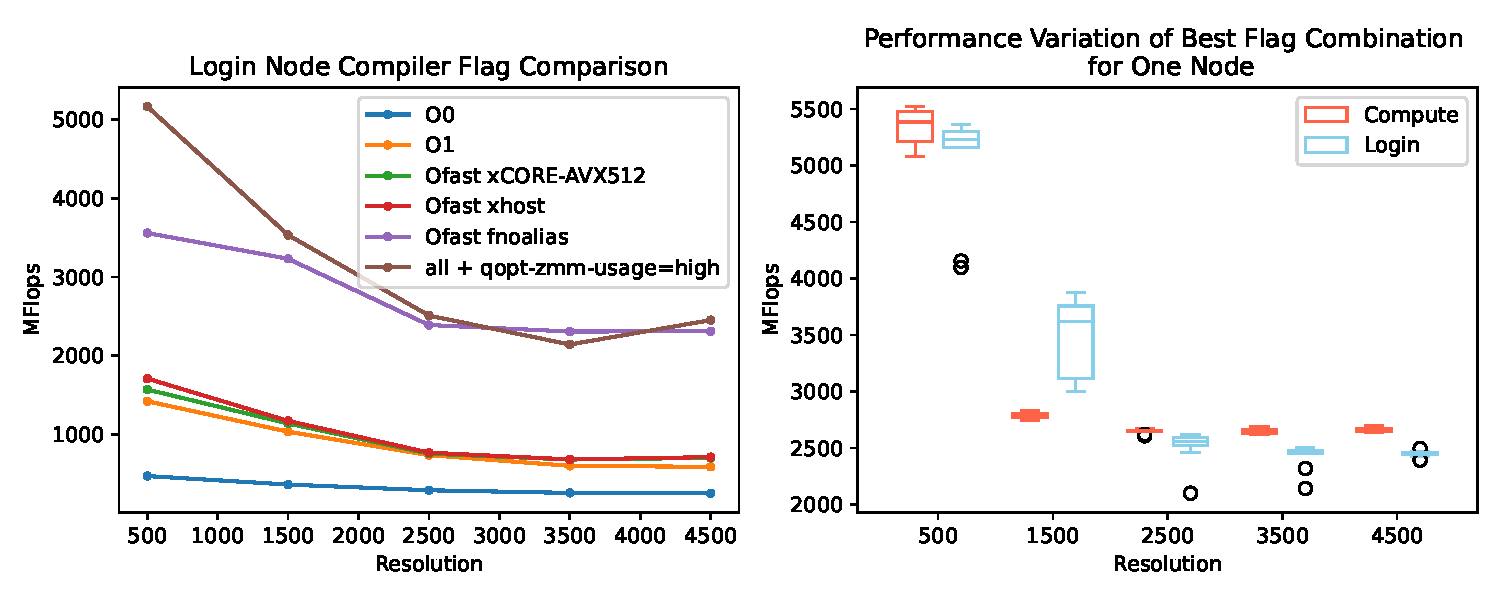
\includegraphics[width=\textwidth]{figures/group2_perf.pdf}
    \caption{Comparison of MFLOPS performance for different compiler flag combinations that had the biggest impact on performance and variation in performance between different runs on login and compute nodes of SUPERMUC-NG (including outliers). Performance was measured for different resolutions (matrix sizes).}
    \label{fig:compiler_flags}
\end{figure}
% "all" means : 0fast xcore fnoalias?

As can be seen in Figure \ref{fig:compiler_flags}, the flag that had the biggest impact on performance was \texttt{-fno-alias}. This flag enabled the compiler to perform a loop interchange in the iteration over the matrix in the Jacobi relaxation method. This improved cache locality by making the fast index row-wise (C language is row-major).

In addition, the general optimization flag \texttt{-O1} had a significant impact compared to the baseline \texttt{-O0} flag: while the first does not, the second includes some speed optimizations.

Lastly, the variation in performance on the login node is much higher than on the compute node, as shown in Figure \ref{fig:compiler_flags}. This is expected, as the login node handles more tasks, leading to increased performance variability.